\documentclass[aspectratio=169]{beamer}

\usetheme{Madrid}
\usecolortheme{beaver}
\setbeamertemplate{navigation symbols}{}
\setbeamertemplate{footline}[frame number]

\usepackage{tikz}
\usetikzlibrary{shapes.geometric, arrows.meta, positioning, calc}
\usepackage{booktabs}
\usepackage{listings}
\usepackage{xcolor}

\definecolor{zentro-red}{RGB}{200, 50, 50}
\definecolor{code-bg}{RGB}{240, 240, 240}

\lstset{
    basicstyle=\ttfamily\small,
    backgroundcolor=\color{code-bg},
    frame=single,
    breaklines=true,
    keywordstyle=\color{blue},
    stringstyle=\color{green!50!black},
}

\title{Context-Aware QA System}
\subtitle{RAG for constrained local environments}
\author{Maxime Pires}
\date{December 16, 2025}

\begin{document}

\begin{frame}
    \titlepage
    \centering
\end{frame}

\begin{frame}{Overview}
    \tableofcontents
\end{frame}

\section{Context \& Constraints}

\begin{frame}{Context-Aware QA Challenge}
    \textbf{Goal:} Intelligent selection of relevant context for a constrained local LLM.
    
    \vspace{1em}
    \textbf{Constraints:}
    \begin{enumerate}
        \item \textbf{Tiny LLM:} 1.8-2B parameters.
        \item \textbf{Context Window:} 1024 tokens max.
    \end{enumerate}
    \vspace{1em}
    \begin{block}{Focus}
        \begin{itemize}
            \item High-Precision Retrieval (Filtering noise).
            \item Smart Context Budgeting (Maximizing density).
        \end{itemize}
    \end{block}
\end{frame}

\begin{frame}{Global Architecture Overview}
    \centering
    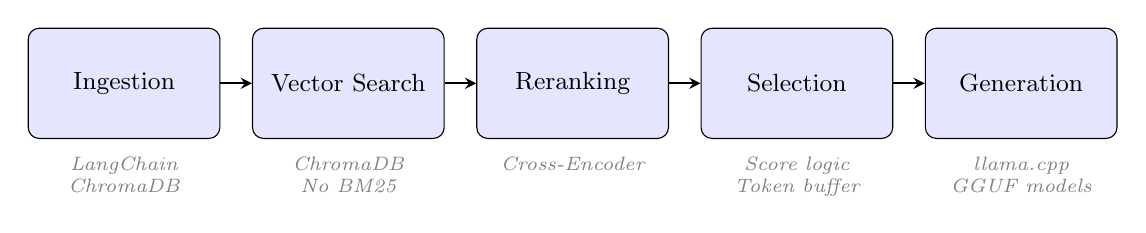
\begin{tikzpicture}[
        node distance=0.6cm and 0.4cm,
        auto,
        block/.style={rectangle, draw, fill=blue!10, text width=2.2cm, text centered, rounded corners, minimum height=1.4cm, font=\small},
        tech/.style={text width=2.2cm, text centered, font=\scriptsize\itshape, text=gray},
        arrow/.style={thick,->,>=stealth}
    ]

        \node [block] (ingest) {Ingestion};
        \node [tech, below=0.1cm of ingest] {LangChain\\ChromaDB};
        \node [block, right=of ingest] (search) {Vector Search};
        \node [tech, below=0.1cm of search] {ChromaDB\\No BM25};
        \node [block, right=of search] (rerank) {Reranking};
        \node [tech, below=0.1cm of rerank] {Cross-Encoder};
        \node [block, right=of rerank] (select) {Selection};
        \node [tech, below=0.1cm of select] {Score logic\\Token buffer};
        \node [block, right=of select] (gen) {Generation};
        \node [tech, below=0.1cm of gen] {llama.cpp\\GGUF models};

        \draw [arrow] (ingest) -- (search);
        \draw [arrow] (search) -- (rerank);
        \draw [arrow] (rerank) -- (select);
        \draw [arrow] (select) -- (gen);
    \end{tikzpicture}
\end{frame}

\section{The RAG Pipeline}

\begin{frame}{Ingestion}
    \textbf{Goal:} Transform raw Markdown into context-rich vectors.
    \vspace{1em}
    \begin{enumerate}
        \item \textbf{Preprocessing:}
        \begin{itemize}
            \item Clean files.
        \end{itemize}
        \vspace{0.5em}
        \item \textbf{Structure-Aware Chunking:}
        \begin{itemize}
          \item \textbf{Tech:} LangChain \texttt{MarkdownHeaderTextSplitter}.
          \item \textbf{Strategy:} Context injection, Document-as-a-Chunk.
        \end{itemize}
        \vspace{0.5em}
        \item \textbf{Vector Storage:}
        \begin{itemize}
            \item \textbf{Embedding:} \texttt{HuggingFaceEmbeddings} (all-mpnet-base-v2).
            \item \textbf{Store:} \texttt{Chroma} (Persistent Local DB).
        \end{itemize}
    \end{enumerate}
\end{frame}

\begin{frame}{Pipeline Step 1: Retrieval}
    \textbf{Architecture:} Vector Search (ChromaDB) with \texttt{all-mpnet-base-v2}.
    
    \vspace{1em}
    \textbf{Strategy:} Retrieve \textbf{Top-20} documents.
    
    \vspace{1em}
    \begin{itemize}
        \item \textbf{MPNet vs MiniLM:} MPNet for higher semantic accuracy, accepting slightly higher latency.
        \item \textbf{Hybrid Search (BM25):} VIP Strategy (disabled by default).
    \end{itemize}
\end{frame}

\begin{frame}{Pipeline Step 2: Reranking}
    \textbf{Architecture:} Cross-Encoder (\texttt{bge-reranker}).
    \vspace{1em}
    \begin{alertblock}{Strict score thresholding}
        Documents below a specific score are discarded (e.g. $< 0.03$).
    \end{alertblock}
    \begin{itemize}
        \item Tiny LLMs are susceptible to "context flooding".
        \item We prefer an empty context (triggering "Insufficient Info") over a noisy one.
    \end{itemize}
\end{frame}

\begin{frame}{Pipeline Step 3: Token Management}
    \textbf{Challenge:} The 1024 limit is a hard crash limit.

    \vspace{1em}
    \textbf{Greedy Selection with Safety Buffer}
    \begin{enumerate}
        \item Target: \textbf{1000 tokens} (leaving 24 for safety).
        \item \texttt{DOC\_SEPARATOR} strategy.
        \item \textbf{Atomic Chunks:} Either a document is fully included or skipped.
    \end{enumerate}
\end{frame}

% --- Slide: Generation (Model Choice) ---
\begin{frame}{Pipeline Step 4: Generation \& Model Choice}
  \textbf{Selection criteria} (Open LLM Leaderboard):
    \begin{itemize}
        \item \textbf{IFEval (Instruction Following):} Critical for strict "No Outside Knowledge" rules.
        \item \textbf{BBH (Reasoning):} For handling contradictory documents.
        \item \textbf{MuSR (Multistep Reasoning):} Hard for tiny models.
    \end{itemize}
    
    \vspace{1em}
    \textbf{Findings:}
    \begin{itemize}
        \item A strong average across all metrics performs better than a single maxed-out score.
        \item Professional LLMs seems to perform better.
        \item Qwen 2.5 offers the best balance.
    \end{itemize}
\end{frame}

\section{Evaluation \& Findings}

\begin{frame}{Evaluation}
    \textbf{Strategy:} "LLM-as-a-Judge" Pipeline.

    \begin{itemize}
        \item \textbf{Judge Model:} Gemini 2.5 Flash.
        \item \textbf{Ground Truth:} Answers generated by Gemini 3.0 Pro.
    \end{itemize}
    \vspace{1em}
    \textbf{Metrics:}
    \begin{itemize}
        \item \textbf{Correctness (1-5):} Does the answer match the Ground Truth meaning?
        \item \textbf{Completeness (1-5):} Are all key details (e.g. specific steps) present?
        \item \textbf{Recall (1-5):} Did the system retrieve the expected sources?
        \item \textbf{Precision (1-5):} Is the context "diluted" with too many irrelevant files?
        \item \textbf{Hallucination (Bool):} Did the model invent procedures not in the source?
    \end{itemize}
    \vspace{1em}
    \textbf{Key findings:}
    \begin{enumerate}
        \item \textbf{Reranking is vital} (context flooding).
        \item \textbf{Strict prompt} (avoid hallucinations).
    \end{enumerate}
\end{frame}

\section{Future Improvements}

\begin{frame}{Bonus: Deployment Architecture (Production)}
    \centering
    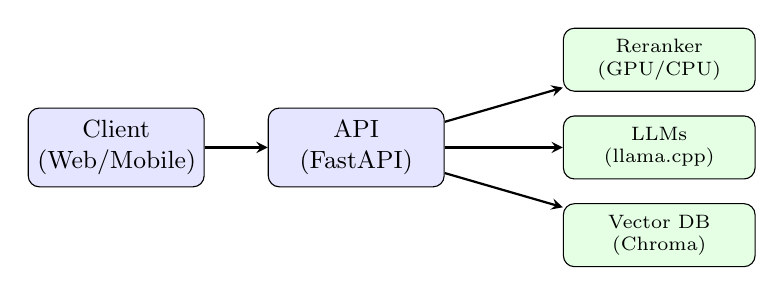
\begin{tikzpicture}[
        node distance=0.8cm,
        auto,
        block/.style={rectangle, draw, fill=blue!10, text width=2cm, text centered, rounded corners, minimum height=1cm, font=\small},
        service/.style={rectangle, draw, fill=green!10, text width=2.2cm, text centered, rounded corners, minimum height=0.8cm, font=\scriptsize},
        arrow/.style={thick,->,>=stealth}
    ]
        \node [block] (client) {Client\\(Web/Mobile)};
        \node [block, right=of client] (gateway) {API\\(FastAPI)};
        
        \node [service, right=1.5cm of gateway] (llm) {LLMs\\(llama.cpp)};
        \node [service, above=0.3cm of llm] (rerank) {Reranker\\(GPU/CPU)};
        \node [service, below=0.3cm of llm] (db) {Vector DB\\(Chroma)};

        \draw [arrow] (client) -- (gateway);
        \draw [arrow] (gateway) -- (rerank);
        \draw [arrow] (gateway) -- (llm);
        \draw [arrow] (gateway) -- (db);
        
    \end{tikzpicture}

    \vspace{2em}
    \textbf{Production Ready Architecture:}
    \begin{itemize}
        \item \textbf{Microservices:} Each component (Reranker, LLM) is an independent Docker container.
        \item \textbf{Scalability:} We can scale the \textit{LLM Workers} horizontally without touching the DB.
        \item \textbf{Robustness:} Prometheus for monitoring latency.
    \end{itemize}
\end{frame}

\begin{frame}{Future Improvements}
    \begin{enumerate}
        \item \textbf{GraphRAG:} To solve "multi-hop" questions (e.g. linking a Policy to a specific Person).
        \item \textbf{Dynamic Thresholding:} Adjusting filters based on query complexity rather than a fixed score.
        \item \textbf{Hardware Acceleration:} GPU for bigger LLMs.
    \end{enumerate}
\end{frame}

\end{document}
